\documentclass{beamer}
\usepackage[size=custom, width=120, height=140, scale=1.5]{beamerposter}

% délky
\newlength{\head}
\setlength{\head}{20cm}

\newlength{\sep}
\setlength{\sep}{1.5cm}\newlength{\vyska}

\setlength{\vyska}{\paperheight}
\addtolength{\vyska}{-\head}

\newlength{\vyskaA}
\setlength{\vyskaA}{\vyska}
\addtolength{\vyskaA}{-2\sep}

\newlength{\vyskaB}
\setlength{\vyskaB}{\vyska}
\addtolength{\vyskaB}{-\sep}

\newlength{\vyskaC}
\setlength{\vyskaC}{\vyska}
\addtolength{\vyskaC}{-3\sep}

\newlength{\side}
\setlength{\side}{30cm}
\addtolength{\side}{-2\sep}

\newlength{\main}
\setlength{\main}{60cm}
\addtolength{\main}{-2\sep}

\newlength{\newparskip}
\setlength{\newparskip}{12pt}

% témata
\usetheme{Rochester}
\usecolortheme{seahorse}

\setbeamerfont{block title}{series=\bfseries,size=\huge}

% odsazení nahoře
\setbeamertemplate{headline}{%
\leavevmode%
  \hbox{%
    \begin{beamercolorbox}[wd=\paperwidth,ht=\head,dp=1.125ex]{white}%
    \insertsectionnavigationhorizontal{\paperwidth}{}{\hskip0pt plus1filll}
    \end{beamercolorbox}%
  }
}

% balíčky
\usepackage{../socstyle}
\usepackage{printlen}
\usepackage{tcolorbox}
\def\asydir{asy}

\usepackage[backend=biber, url=true, sorting=none]{biblatex}

\usepackage{url}
\addbibresource{/home/adam/tex/soc.bib}

% asi naprd definice
\title{Mechanika rodin planetek \\ s aplikací na rodinu Eunomia}
\author{Adam Křivka \\ \and doc. Mgr. Miroslav Brož, Ph.\,D.}
\institute{Cyrilometodějské gymnázium a střední odborná škola pedagogická Brno,\\ Lerchova 63, 602 00 Brno}

\begin{document}
\begin{frame}
\begin{columns}[t]

\begin{column}{\sep}
\end{column}
\begin{column}{\side}
	\begin{minipage}[t][0.5\vyskaA][t]{\textwidth}
		\begin{block}{Úvod\phantom{Úy}}
			Planetky jsou nejpočetnější a svým způsobem nejzajímavější skupinou těles ve~sluneční soustavě. První planetka byla objevena v roce 1801, v dnešní době je již známo přes půl milionu planetek.\\[\newparskip]

%(konkrétně souborný katalog použit v~této práci \cite{astorb}\cite{knezevic12}\cite{nugent15}\cite{usui11}\cite{ivezic01} obsahuje 524\,138 položek).

			V~hlavním pásu planetek mezi Marsem a~Jupiterem tvoří planetky rodiny --- skupiny vzniklé rozpadem stejného mateřského tělesa, způsobým srážkou s~jiným tělesem. V~naší práci se budeme soustředit na početnou rodinu Eunomia, nacházející se ve středním hlavním pásu.\\[\newparskip]

			Studiem kolizních rodin můžeme zjistit mnoho informací o~vzniku sluneční soustavy a~její dynamické struktuře, např. můžeme podpořit teorii o~\textit{Velkém pozdním bombardování} (angl. \textit{Late Heavy Bombardment})~\cite{broz13}.\\[\newparskip]
			\begin{figure}[!htb]
				\centering
				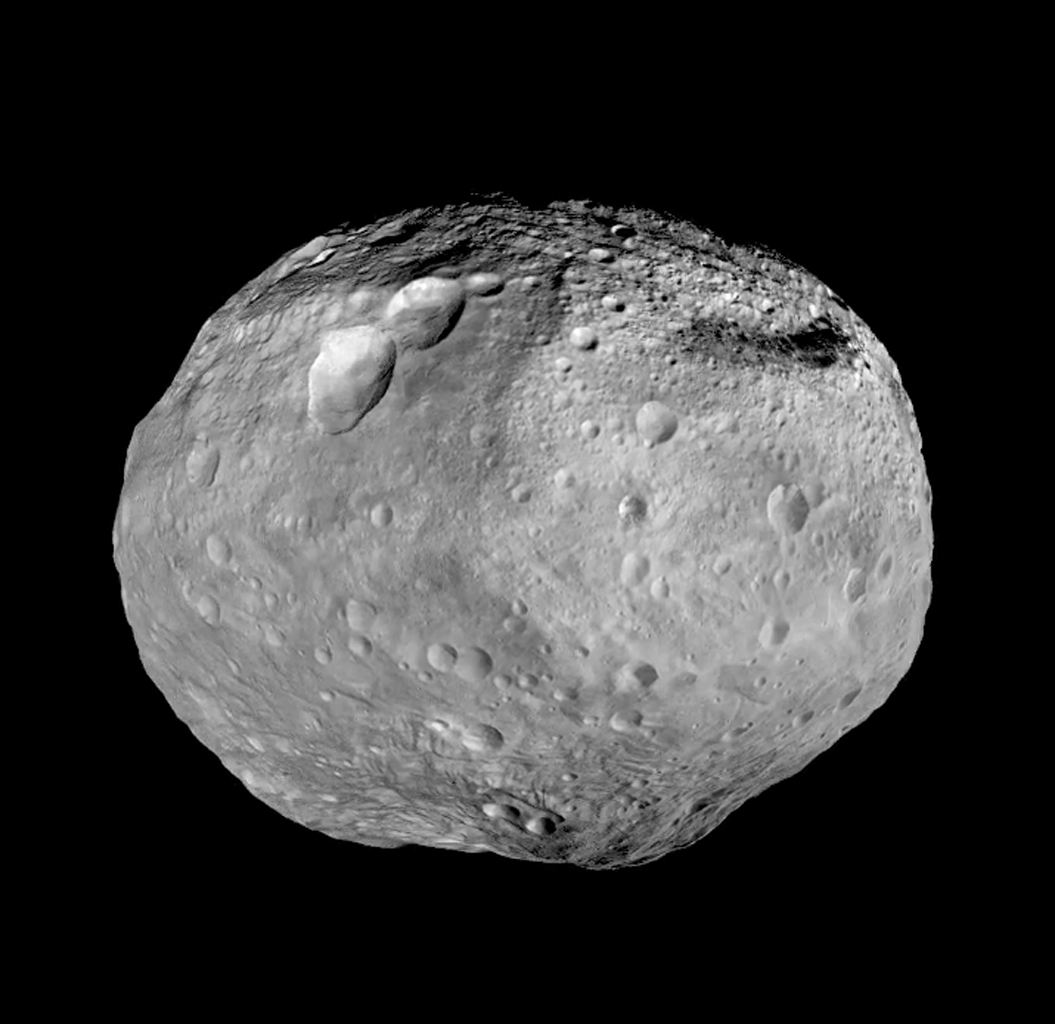
\includegraphics[width=0.6\textwidth]{../obr/vesta.jpg}
				\caption{Planetka (4) Vesta --- druhé největší a~nejhmotnější těleso hlavního pásu planetek. Fotografie byla pořízena sondou \textit{Dawn}. Převzato z~\cite{jplvesta}.} \label{fig:vesta}
			\end{figure}
		\end{block}
	\end{minipage}

	\vspace{\sep}

\begin{tcolorbox}
ahooj
\end{tcolorbox}
	\begin{minipage}[t][0.5\vyskaA][t]{\textwidth}
		\begin{block}{Metody\phantom{Úy}}
			\begin{figure}[!htb]
				\centering 
				{\Huge \asyinclude[width=0.9\textwidth]{../asy/f_euler.asy}}
				% \asyinclude{../asy/b_euler.asy}
				\caption{Ilustrace dopředné Eulerovy integrační metody pro dvě tělesa, kdy větší těleso (velká tečka vlevo) gravitačně působí na menší těleso (malé tečky vpravo). Jsou ukázány první tři iterace. Algoritmus byl doopravdy implementován, s~počátečními hodnotami: $h=20\,{\rm \text{dnů}}$, $m_1=2\cdot10^{30}\,{\rm kg}$, $G=6,67\cdot10^{-11}\,{\rm m^3\,kg^{-1}\,s^{-2}}$, $|\vec{r}_0|=1\,{\rm AU}$, $v_0=29\,861\,{\rm m\,s^{-1}}$. Vektory jsou vhodně škálované. Šedá křivka znázorňuje analytické řešení problému dvou těles.} \label{fig:euler}
			\end{figure}
		\end{block}
	\end{minipage}

	\vspace{\sep}

\end{column}

\begin{column}{2\sep}
\end{column}

\begin{column}{\main}
\uselengthunit{mm}\printlength{\vyskaA}
	\begin{block}{Výsledky\phantom{Úy}}
		\begin{minipage}[t][1.0\vyskaB][t]{\textwidth}
			\begin{figure}
				\centering
				\begin{subfigure}[t]{0.3\textwidth}
					\centering
					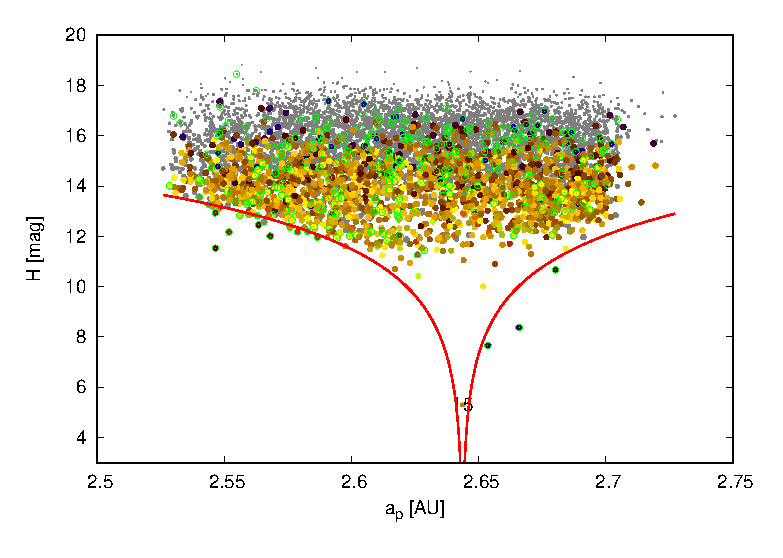
\includegraphics[width=1.0\textwidth]{../obr/aH_wise}
					\caption{Rozdělení pozorované rodiny Eunomia v~rovině vlastní hlavní poloosy $a_{\rm p}$ a~absolutní hvězdné velikosti $H$. Barevná škála byla zvolnea dle~katalogu WISE. Šedá křivka označuje funkci s~parametry ${C=2,2\cdot10^{-4}}$ a~${a_{\rm c}=2,643666\,{\rm AU}}$ a~červená křivka označuje posunutou funkci s~parametry ${C=2\cdot10^{-4}}$ a~${a_{\rm c}=2,641666\,{\rm AU}}$. K~odstranění  jsme zvolili červenou funkci. Lze pozorovat typický tvar \uv{V}, který je způsobem počátečním rychlostním polem a~Jarkovského jevem, jenž je ještě zesílen vlivem YORPu, což způsobuje zvýšenou koncentraci malých planetek při okrajích rodiny.}
					\label{fig:aH_wise}
				\end{subfigure}
				\begin{subfigure}[t]{0.3\textwidth}
					\centering
					\includegraphics[width=1.0\textwidth]{../obr/pV_pIR}
					\caption{Albeda $p_{\rm V}$ (ve viditelném spektru) a~$p_{\rm IR}$ (v~infračerveném spektru) z~katalogu WISE \cite{nugent15}. Barevná škála byla taktéž převzata z~katalogu WISE, barvy neodpovídají reálnému zbarvení. Zelené kroužky označují přimísená tělesa vyřazená jakoukoliv z~použitých metod. Pro vyřazení přimísených těles touto metodou byly zvoleny hraniční hodnoty $0,05 \leq p_{\rm V} \leq 0,4$.}
					\label{fig:pV_pIR}
				\end{subfigure}
				\begin{subfigure}[t]{0.3\textwidth}
					\centering
					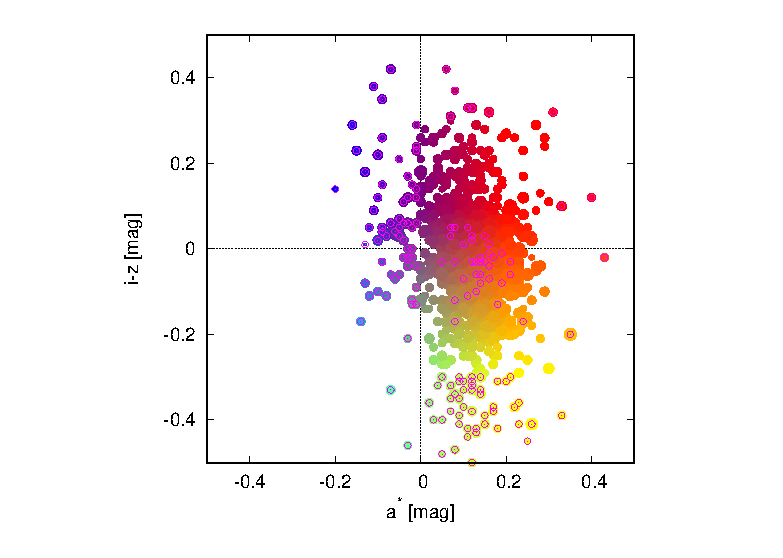
\includegraphics[width=1.0\textwidth]{../obr/astar_iz}
					\caption{Barevné indexy $a^*$ a~$i-z$ z~katalogu Sloan \cite{ivezic01}. Barevná škála byla taktéž zvolena dle~katalogu Sloan, barvy neodpovídají reálnému zbarvení. Zelené kroužky označují přimísená tělesa vyřazená jakoukoliv z~použitých metod. Pro vyřazení přimísených těles byly zvoleny hraniční hodnoty $0\leq a^* \leq 0,3$ a~$-0,3\leq i-z \leq 0,3$.}
					\label{fig:astar_iz}
				\end{subfigure}
			\end{figure}

			\begin{figure}
				\centering
				\begin{subfigure}[t]{0.49\textwidth}
				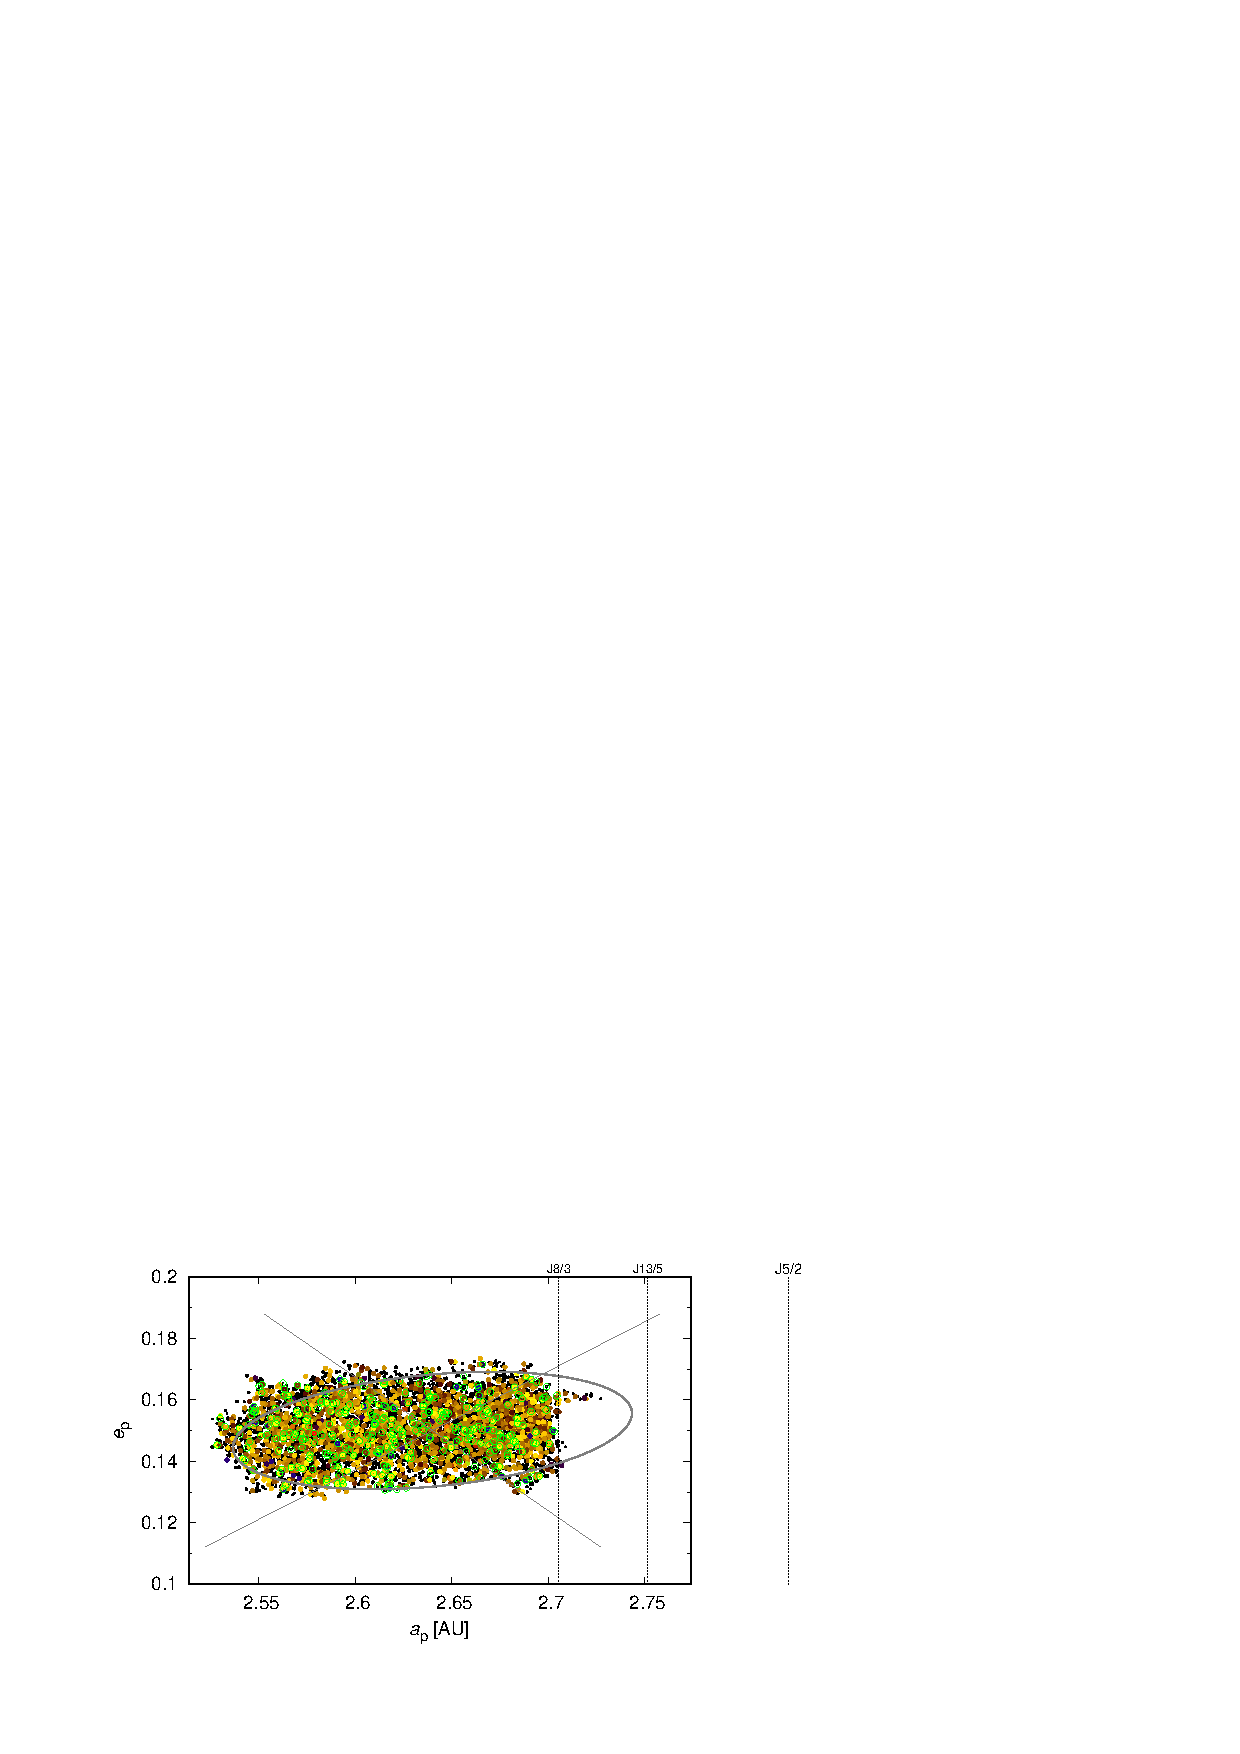
\includegraphics[width=1.0\textwidth]{../obr/ae_wise}
				\end{subfigure}
				\begin{subfigure}[t]{0.49\textwidth}
				\includegraphics[width=1.0\textwidth]{../obr/ai_wise}
				\end{subfigure}
				\caption{Pozorovaná rodina Eunomia pro hraniční rychlost $v_{\rm cutoff} = 44\,{\rm m/s}$ v~rovině vlastní hlavní poloosy $a_{\rm p}$ a~vlastní excentricity $e_{\rm p}$ (nahoře) a~v~rovině vlastní hlavní poloosy $a_{\rm p}$ a~vlastního sklonu $\sin I_{\rm p}$ (dole). Barevná škála odpovídá albedu $p_{\rm V}$ a~$p_{\rm IR}$ z~katalogu WISE\@. Nápisy J8/3 a~J13/5 označují polohu rezonancí středního pohybu s~Jupiterem. Šedé elipsy a~úsečky (degenerované elipsy) naznačují výpočet Gaussových rovnic pro hodnoty pravé anomálie $f=0^\circ,\,90^\circ,\,180^\circ$ (nahoře) a~součtu $\omega+f=0^\circ,\, 50^\circ,\, 90^\circ$ (dole), kde zvolenou tučnější elipsou je elipsa pro hodnoty $f=90^\circ$ a~$\omega+f=50^\circ$.}
				\label{fig:ae_ai_wise}
			\end{figure}

			\immediate\write18{convert -trim -transparent white ../obr/ae_5.png ../obr/ae_5t.png}
			\immediate\write18{convert -trim -transparent white ../obr/ae_105.png ../obr/ae_105t.png}
			\immediate\write18{convert -trim -transparent white ../obr/ae_405.png ../obr/ae_405t.png}
			\immediate\write18{convert -trim -transparent white ../obr/ae_905.png ../obr/ae_905t.png}
			\begin{figure}[t]
				\centering
				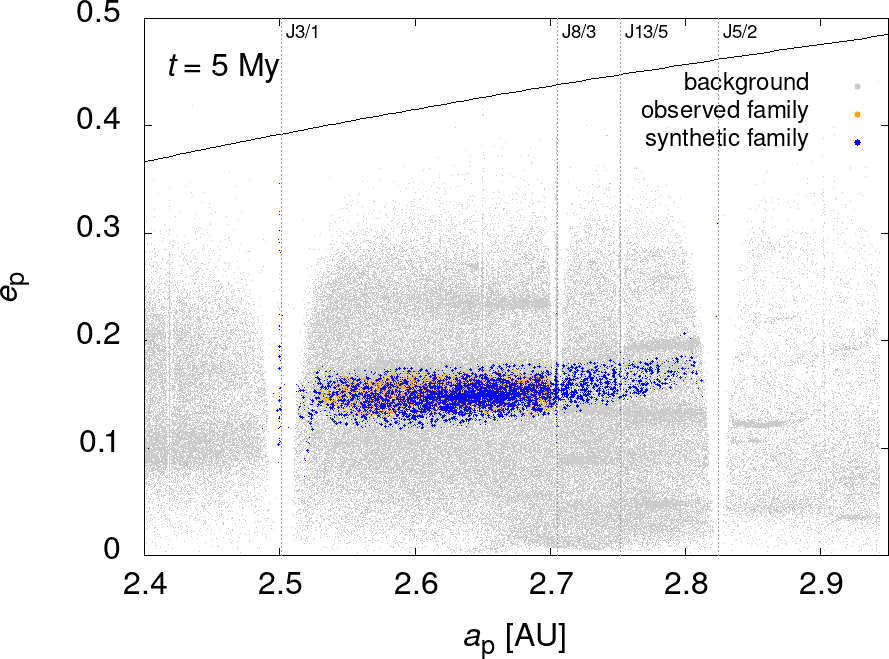
\includegraphics[width=0.49\textwidth]{../obr/ae_5t.png}
				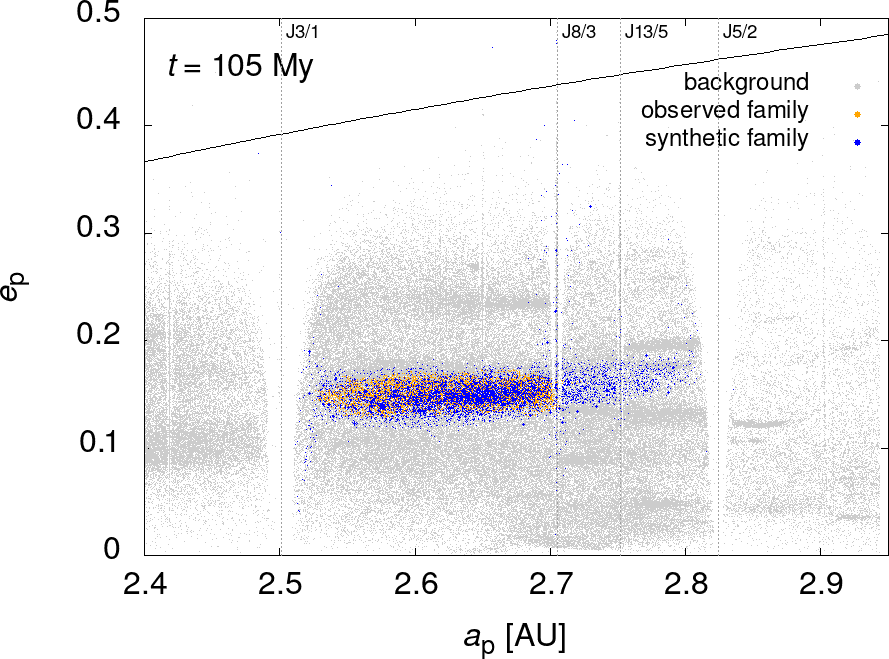
\includegraphics[width=0.49\textwidth]{../obr/ae_105t.png}\\
				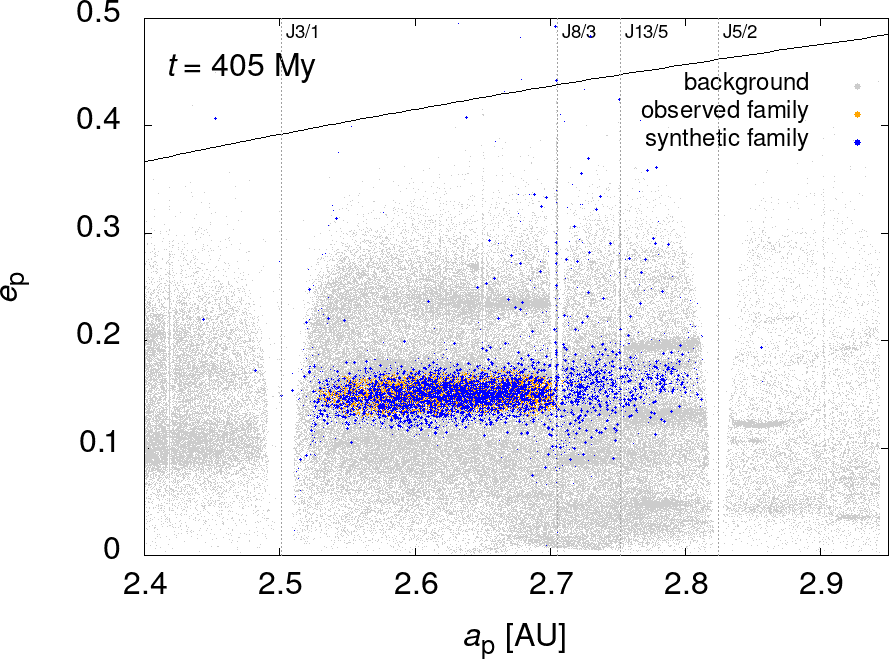
\includegraphics[width=0.49\textwidth]{../obr/ae_405t.png}
				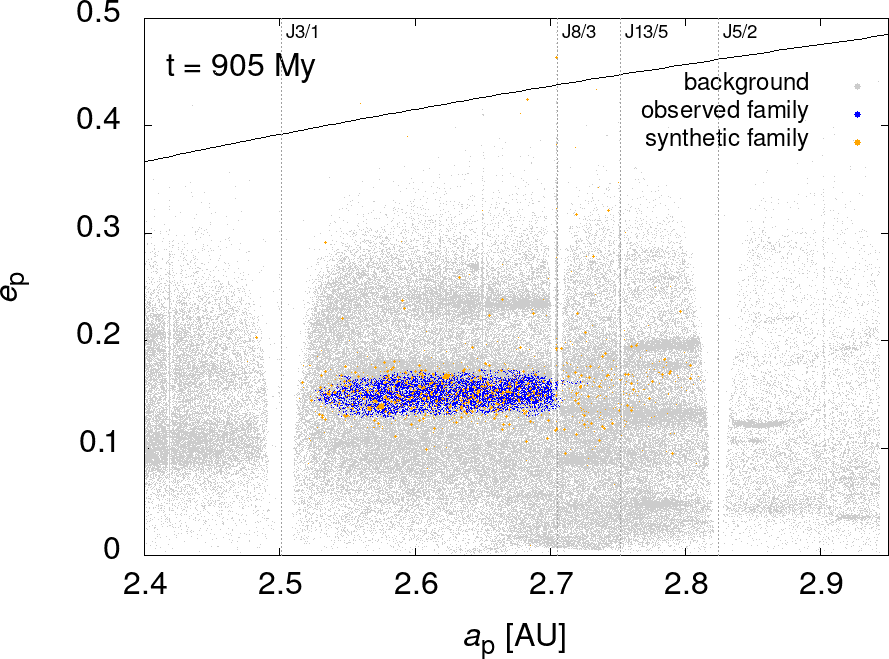
\includegraphics[width=0.49\textwidth]{../obr/ae_905t.png}
				\caption{Výsledky simulace v~prostoru $(a_{\rm p},\,e_{\rm p})$ v~časech postupně $t=5,\,105,\,405,\,905$ miliónů let. Modré body označují simulovanou rodinu, žluté body pozorovanou rodinu identifikovanou HCM a~šedé body pozadí a~jiné okolní rodiny. Jsou také značeny nejvýznamnější rezonance s~Jupiterem J3/1, J8/3, J13/5 a~J5/2. Černá křivka nahoře označuje hranici oblasti, kde je hlavní poloosa a~excentricita tělesa taková, že dráha kříží dráhu Marsu. Podobná hranice existuje i~pro Jupiter, ale ta se nachází mimo tyto grafy (přibližně kolem $e=0,65$). Skripty k~vytvoření těchto grafů můžete nalézt v~příloze \ref{app:fig:ae_sim}.} \label{fig:ae_sim}
			\end{figure}	

			\immediate\write18{convert -trim ../obr/ae_chi_0006.png ../obr/ae_chi_0006t.png}
			\immediate\write18{convert -trim ../obr/ae_chi_0106.png ../obr/ae_chi_0106t.png}
			\immediate\write18{convert -trim ../obr/ae_chi_0406.png ../obr/ae_chi_0406t.png}
			\immediate\write18{convert -trim ../obr/ae_chi_empty.png ../obr/ae_chi_emptyt.png}
			\begin{figure}
				\centering
				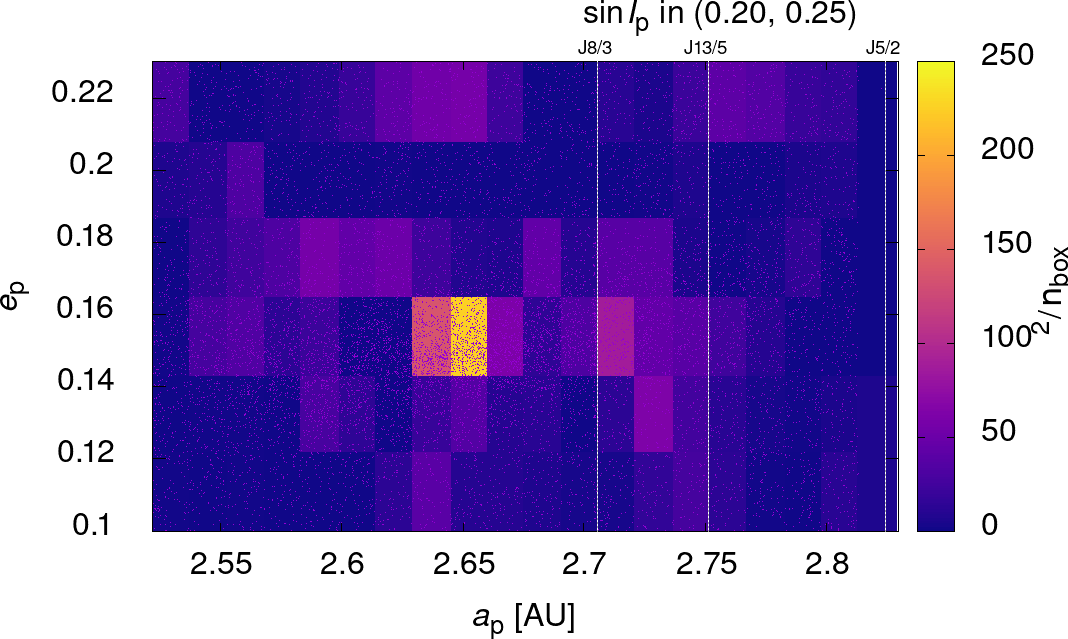
\includegraphics[width=0.49\textwidth]{../obr/ae_chi_0006t.png}
				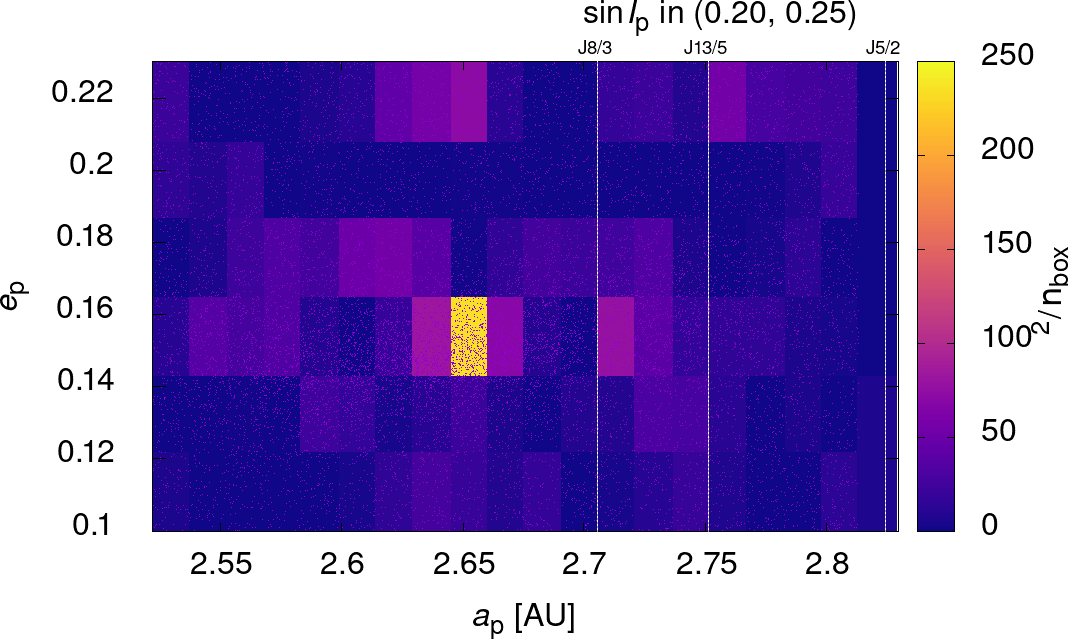
\includegraphics[width=0.49\textwidth]{../obr/ae_chi_0106t.png}\\
				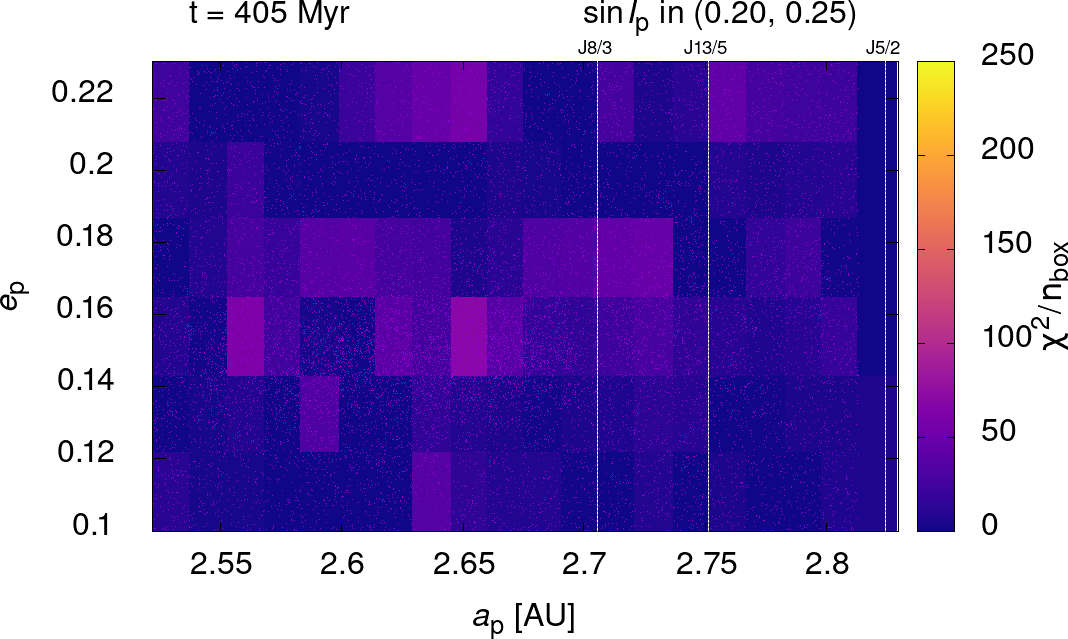
\includegraphics[width=0.49\textwidth]{../obr/ae_chi_0406t.png}
				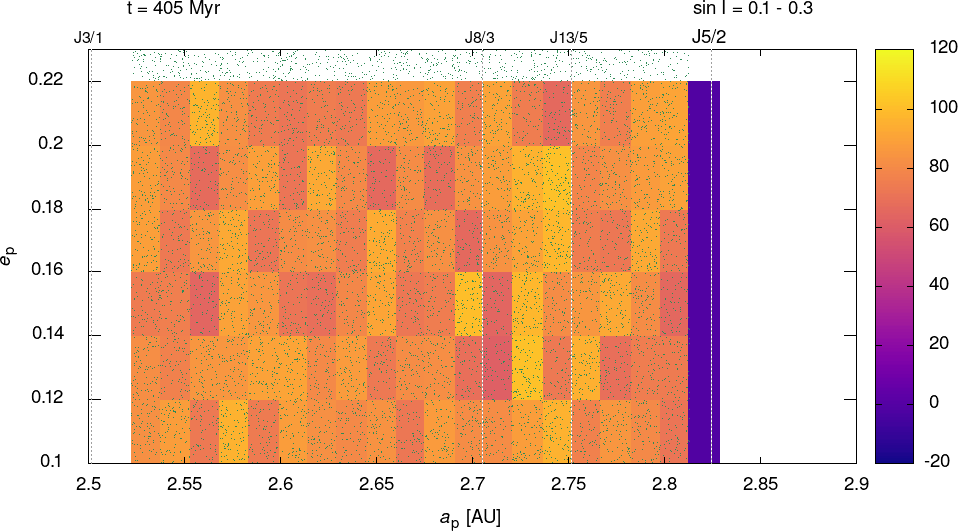
\includegraphics[width=0.49\textwidth]{../obr/ae_chi_emptyt.png}
				\caption{Hodnota chi kvadrátu $\chi^2$ pro každý box v~prostoru $(a,\,e)$. Na prvních třech obrázcích lze vidět rozdělení chi kvadrátu pro $t=5,\,105,\,405$ miliónů let, na posledním obrázku lze vidět rozdělení chi kvadrátu při vygenerování pouze pozadí bez použití částic simulované rodiny. Barevná škála je pro všechny až na poslední obrázek stejná. Zelené tečky označují simulovanou populaci i~s~přidaným pozadím. J8/3, J13/5 a~J5/2 označují rezonance středního pohybu s~Jupiterem.} \label{fig:ae_chi2}
			\end{figure}

		\end{minipage}
	\end{block}
	\vspace{\sep}
\end{column}

\begin{column}{2\sep}
\end{column}

\begin{column}{\side}
	\begin{block}{Závěry\phantom{Úy}}
		\begin{minipage}[t][0.4\vyskaC][t]{\textwidth}
			\begin{figure}
			\centering
			\includegraphics[width=\textwidth]{../obr/ae_scl.png}\\
			\includegraphics[width=\textwidth]{../obr/ae_obs.png}\\
			\caption{Graf $(a_{\rm p}, e_{\rm p})$ pro simulovanou (vlevo) a~pozorovanou (vpravo) rodinu Eunomia v~čase $t=455$ miliónů let, kdy byla hodnota $\chi^2$ nejlepší. Tentokrát barevná škála označuje počet těles v~daném boxu. Lze porovnat s~podobným grafem $\chi^2$ --- problémové oblasti jsou přímo v~centru rodiny (simulovaná populace je příliš kompaktní) a~potom v~oblasti $a_{\rm p}\in(2,55\,{\rm AU};\,2,5\,{\rm AU})$ a~$e_{\rm p}\in(0,14;\,0,16)$, kam se naopak částice simulované populace nestihly rozšířit.} \label{fig:ae_obs_scl}
		\end{figure}

		\end{minipage}
	\end{block}
	\vspace{\sep}
	\begin{block}{Budoucí práce\phantom{Úy}}
		\begin{minipage}[t][0.3\vyskaC][t]{\textwidth}
		\begin{figure}
			\centering
			\includegraphics[width=0.7\textwidth]{../obr/chi2.eps}
			\caption{Závislost redukovaného chí kvadrátu $\chi^2/n_{\rm box}$ na čase $t$. Lze vidět, že se jeho hodnota snižuje, tudíž můžeme předpokládat, že bychom delší integrací dostali nižší hodnoty, případně bychom mohli určit interval stáří rodiny Eunomia.} \label{fig:chi2}
		\end{figure}
		\end{minipage}
	\end{block}
	\vspace{\sep}
	\begin{block}{Reference\phantom{Úy}}

		\printbibliography
		\begin{minipage}[t][0.3\vyskaC][t]{\textwidth}
			{\tiny \printbibliography}
		\end{minipage}
	\end{block}
\end{column}


\begin{column}{\sep}
\end{column}

\end{columns}
\end{frame}
\end{document}
